\newpage 
\section{Архитектура центрального процессора}
\subsection{Архитектура процессоров семейства x86}
Рассмотрим основные архитектурные особенности центрального процессора.
Одни из базовых понятий для производительности процессора:
\begin{itemize}
	\item Latency (Латентность команды) --- это число тактов, необходимое для завершения одной команды с момента готовности входных данных команды(выборки их из памяти) и начало ее выполнения
	\item Throughput (Пропускная способность команды) --- это число тактов ожидания, которое требуется процессору перед запуском на выполнение такой же команды
\end{itemize}   

\subsection{Архитектура процессоров семейства x64}
\subsubsection{Архитектура процессора Intel Core i7 980X}
\noindent{\bf\ttОбзор}\\
Intel Core i7 — семейство процессоров x86-64 Intel. Core i7 980X это процессор семейства Gulftown вышедшего в 2010 году. Основные характеристики представлены с помощью программы cpu-z:
\begin{center}
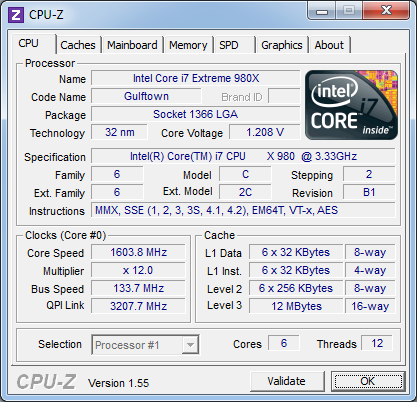
\includegraphics[scale=1]{imgs/cpu-z.png} 
\end{center}

